\documentclass{book}[oneside]
\usepackage{CJKutf8}
\usepackage{amsmath}
\usepackage{amsfonts}
\usepackage{amsthm}
\usepackage{titlesec}
\usepackage{titletoc}
\usepackage{xCJKnumb}
\usepackage{clrscode3e}
\usepackage{ragged2e}
\justifying\let\raggedright\justifying

\usepackage{tikz}
\titleformat{\chapter}{\centering\Huge\bfseries}{第\, \xCJKnumber{\thechapter}\,
    章}{1em}{}
  % \renewcommand{\chaptermark}[1]{\markboth{第 \thechapter 章}{}}
\usepackage{mathrsfs}

\newtheorem{Def}{定义}[chapter]
\newtheorem{Thm}{定理}[chapter]
\newtheorem{Cor}{推论}[chapter]
\newtheorem{Ax}{公理}[chapter]

\newtheorem{Exercise}{练习}[chapter]

\newtheorem{Example}{例}[chapter]


\begin{document}
\begin{CJK*}{UTF8}{gbsn}
  \title{离散数学讲义}
  \author{陈建文}
  \maketitle
  % \tableofcontents
  

  \setcounter{chapter}{5}
  \chapter{图的基本概念}
设$V$为一个集合,$V$的一切二元子集之集合记为$\mathcal{P}_2(V)$,即
\begin{equation*}
  \mathcal{P}_2(V) = \{A|A \subseteq V \text{且} |A| = 2\}\text{。}
\end{equation*}
\begin{Def}
  设$V$为一个非空有限集合,$E \subseteq \mathcal{P}_2(V)$,二元组$G = (V, E)$称为一个无向图。$V$中的元素称为无向图$G$的顶点,$V$为顶点集;$E$中的元素称为无向图$G$的边,$E$为边集。无向图简称图。如果$|V|=p$,$|E|=q$,则称$G$为一个$(p,q)$图,即$G$是一个具有$p$个顶点$q$条边的图。
\end{Def}
      \centering
    \begin{tikzpicture}[auto,
    specification/.style ={circle, draw, thick, inner sep = 0pt, minimum size=2mm}]
   \node[specification] (A)  [label=0:$v_2$] at (18:1.3cm)  {};
   \node[specification] (B)  [label=90:$v_1$] at (90:1.3cm)  {};
   \node[specification] (C)  [label=180:$v_5$] at (162:1.3cm)  {};
   \node[specification] (D) [label=180:$v_4$] at (234:1.3cm)  {};
   \node[specification] (E)  [label=0:$v_3$] at (306:1.3cm)  {};      
   
   
   \draw[thick] (A) to  (B);
   \draw[thick] (B) to  (C);
   \draw[thick] (C) to  (D);
   \draw[thick] (D) to  (E);
   \draw[thick] (E) to  (A);
   \draw[thick] (A) to  (C);
   \draw[thick] (B) to  (E);
   \draw[thick] (C) to  (E);
   \draw[thick] (D) to  (A);
 \end{tikzpicture}

   \begin{Def}
    在图$G=(V,E)$中,如果$\{u,v\}\in E$,则称顶点$u$与$v$邻接;若$x$与$y$是图$G$的两条边,并且仅有一个公共端点,即$|x \cap y|= 1$,则称边$x$与$y$邻接;如果$x=\{u,v\}$是图$G$的一条边,则称$u$与$x$互相关联,同样的,称$v$与$x$互相关联。
  \end{Def}

    \begin{Def}
   如果一个图中两个顶点间允许有多于一条边存在,则称为多重图,这些边称为多重边; 如果一个图中允许联结一个顶点与其自身的边存在,则称为带环图,这些边称为环;允许有环或多重边存在的图,称之为伪图。
  \end{Def}
  \begin{Def}
设$G=(V,E)$为一个图,如果$E=\Phi$,则称$G$为零图; $(1,0)$图称为平凡图。    
  \end{Def}

  \begin{Def}
    设$v$为图$G=(V,E)$的任意一个顶点,$G$中与$v$关联的边的数目称为顶点$v$的度,记为$\deg v$。
  \end{Def}

  \begin{Thm}
    设$G=(V,E)$为一个具有$p$个顶点$q$条边的图,则$G$中各顶点度的和等于边的条数$q$的两倍,即
        \begin{equation*}
      \sum_{v \in V}\deg v = 2q
    \end{equation*}
  \end{Thm}
  \begin{Thm}
       在任一图中,度为奇数的顶点的数目必为偶数。
  \end{Thm}
 \begin{Def}
    图$G$称为$r$度正则图,如果$G$的每个顶点的度都等于$r$。3度正则图也叫三次图。
    一个具有$p$个顶点的$p-1$度正则图称为包含$p$个顶点的完全图,记为$K_p$。
  \end{Def}
  \begin{Def}
    设$G=(V,E)$为一个图,图$H=(V_1,E_1)$称为$G$的一个子图,当且仅当$V_1$为$V$的
    非空子集且$E_1$为$E$的子集。如果$H \neq G$,则称$H$为$G$的真子图。
  \end{Def}
    \begin{minipage}[c]{0.4\textwidth}
\centering
    \begin{tikzpicture}[auto,
    specification/.style ={circle, draw, thick, inner sep = 0pt, minimum size=2mm}]
   \node[specification] (A)  [label=0:$v_2$] at (18:1.3cm)  {};
   \node[specification] (B)  [label=90:$v_1$] at (90:1.3cm)  {};
   \node[specification] (C)  [label=180:$v_5$] at (162:1.3cm)  {};
   \node[specification] (D) [label=180:$v_4$] at (234:1.3cm)  {};
   \node[specification] (E)  [label=0:$v_3$] at (306:1.3cm)  {};      
   
   
   \draw[thick] (A) to  (B);
   \draw[thick] (B) to  (C);
   \draw[thick] (C) to  (D);
   \draw[thick] (D) to  (E);
   \draw[thick] (E) to  (A);
   \draw[thick] (A) to  (C);
   \draw[thick] (B) to  (E);
   \draw[thick] (C) to  (E);
   \draw[thick] (D) to  (A);
 \end{tikzpicture}
\\ \centering G 
    \end{minipage}\hspace{2cm}
    \begin{minipage}[c]{0.4\textwidth}
\centering
    \begin{tikzpicture}[auto,
    specification/.style ={circle, draw, thick, inner sep = 0pt, minimum size=2mm}]
   \node[specification] (A)  [label=0:$v_2$] at (18:1.3cm)  {};
   \node[specification] (B)  [label=90:$v_1$] at (90:1.3cm)  {};
   \node[specification] (E)  [label=0:$v_3$] at (306:1.3cm)  {};      
   
   
   \draw[thick] (A) to  (B);
   \draw[thick] (B) to  (E);
 \end{tikzpicture}
\\ \centering H 
    \end{minipage}

  \begin{Def}
    设$G=(V,E)$为一个图,如果$F\subseteq E$,则称$G$的子图$H=(V,F)$ 为$G$的一个生成子图。
  \end{Def}
  \begin{minipage}[c]{0.4\textwidth}
    \centering
    \begin{tikzpicture}[auto,
    specification/.style ={circle, draw, thick, inner sep = 0pt, minimum size=2mm}]
   \node[specification] (A)  [label=0:$v_2$] at (18:1.3cm)  {};
   \node[specification] (B)  [label=90:$v_1$] at (90:1.3cm)  {};
   \node[specification] (C)  [label=180:$v_5$] at (162:1.3cm)  {};
   \node[specification] (D) [label=180:$v_4$] at (234:1.3cm)  {};
   \node[specification] (E)  [label=0:$v_3$] at (306:1.3cm)  {};      
   
   
   \draw[thick] (A) to  (B);
   \draw[thick] (B) to  (C);
   \draw[thick] (C) to  (D);
   \draw[thick] (D) to  (E);
   \draw[thick] (E) to  (A);
   \draw[thick] (A) to  (C);
   \draw[thick] (B) to  (E);
   \draw[thick] (C) to  (E);
   \draw[thick] (D) to  (A);
 \end{tikzpicture}
\\ \centering G 
    \end{minipage}\hspace{2cm}
    \begin{minipage}[c]{0.4\textwidth}
\centering
    \begin{tikzpicture}[auto,
    specification/.style ={circle, draw, thick, inner sep = 0pt, minimum size=2mm}]
   \node[specification] (A)  [label=0:$v_2$] at (18:1.3cm)  {};
   \node[specification] (B)  [label=90:$v_1$] at (90:1.3cm)  {};
   \node[specification] (C)  [label=180:$v_5$] at (162:1.3cm)  {};
   \node[specification] (D) [label=180:$v_4$] at (234:1.3cm)  {};
   \node[specification] (E)  [label=0:$v_3$] at (306:1.3cm)  {};      
   
   
   \draw[thick] (A) to  (B);
   \draw[thick] (B) to  (E);
 \end{tikzpicture}
 \\ \centering H
    \end{minipage}

  \begin{Def}
    设图$G$的子图$H$具有某种性质,若$G$中不存在与$H$不同的具有此性质且包含$H$的子图,则称$H$是具有此性质的极大子图。
  \end{Def}
  \begin{Def}
    设$S$为图$G=(V,E)$的顶点集$V$的非空子集,则$G$的以$S$为顶点集的极大子图称为由$S$导出的子图,记为$\langle S \rangle$。
形式的,
\begin{equation*}
  \langle S \rangle=(S, \mathcal{P}_2(S) \cap E)
\end{equation*}
  \end{Def}
    \begin{minipage}[c]{0.4\textwidth}
    \centering
    \begin{tikzpicture}[auto,
    specification/.style ={circle, draw, thick, inner sep = 0pt, minimum size=2mm}]
   \node[specification] (A)  [label=0:$v_2$] at (18:1.3cm)  {};
   \node[specification] (B)  [label=90:$v_1$] at (90:1.3cm)  {};
   \node[specification] (C)  [label=180:$v_5$] at (162:1.3cm)  {};
   \node[specification] (D) [label=180:$v_4$] at (234:1.3cm)  {};
   \node[specification] (E)  [label=0:$v_3$] at (306:1.3cm)  {};      
   
   
   \draw[thick] (A) to  (B);
   \draw[thick] (B) to  (C);
   \draw[thick] (C) to  (D);
   \draw[thick] (D) to  (E);
   \draw[thick] (E) to  (A);
   \draw[thick] (A) to  (C);
   \draw[thick] (B) to  (E);
   \draw[thick] (C) to  (E);
   \draw[thick] (D) to  (A);
 \end{tikzpicture}
 \\ \centering G 
    \end{minipage}\hspace{2cm}
    \begin{minipage}[c]{0.4\textwidth}
    \centering
    \begin{tikzpicture}[auto,
    specification/.style ={circle, draw, thick, inner sep = 0pt, minimum size=2mm}]
   \node[specification] (A)  [label=0:$v_2$] at (18:1.3cm)  {};
   \node[specification] (B)  [label=90:$v_1$] at (90:1.3cm)  {};
   \node[specification] (E)  [label=0:$v_3$] at (306:1.3cm)  {};      
   
   
   \draw[thick] (A) to  (B);
   \draw[thick] (E) to  (A);
   \draw[thick] (B) to  (E);
 \end{tikzpicture}
\\ \centering H 
    \end{minipage}
  \begin{Def}
    设$G=(V,E)$, $H = (U, F)$为两个图,如果存在一个一一对应$\phi:V \to
    U$,使得$\{u,v\} \in E$当且仅当$\{\phi(u),\phi(v)\} \in F$,则称$G$与$H$同构。
  \end{Def}
    \begin{minipage}[c]{0.4\textwidth}
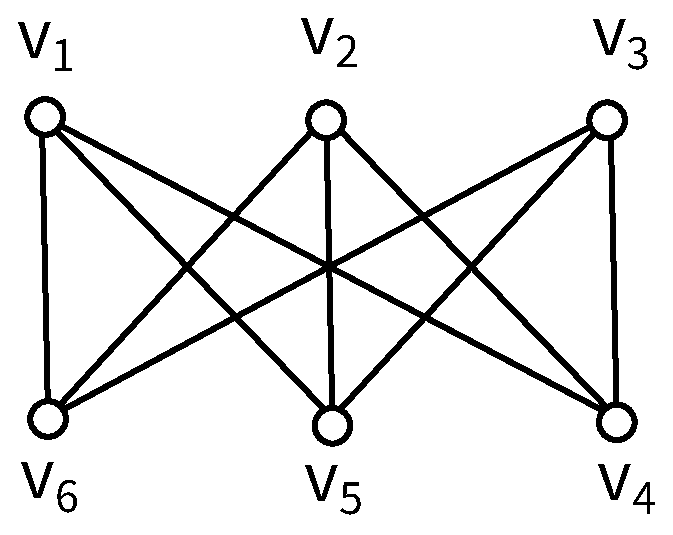
\includegraphics[width=4cm,height=3cm]{k33} \\ \centering G 
    \end{minipage}\hspace{2cm}
    \begin{minipage}[c]{0.4\textwidth}
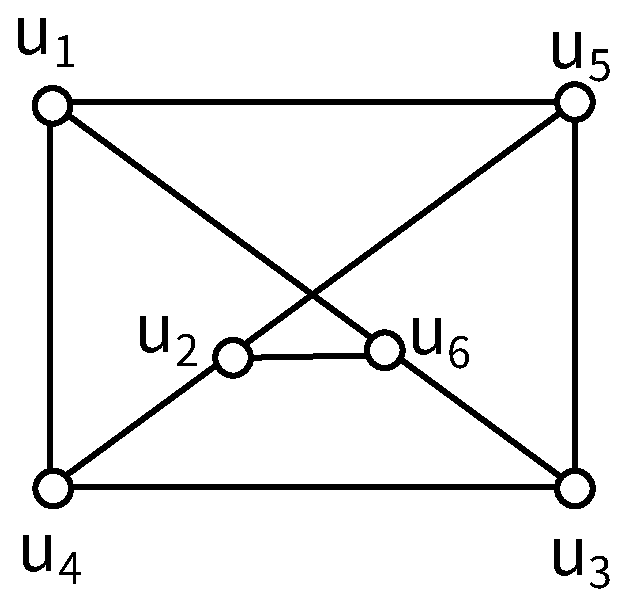
\includegraphics[width=4cm,height=3cm]{isomorphic} \\ \centering H 
    \end{minipage}
  \begin{Def}
    设$G=(V,E)$为一个图。$G$的一条{\bfseries 通道}为$G$的顶点和边的一个交错序列
    \[v_0,x_1,v_1,x_2,v_2,x_3,\ldots,v_{n-1},x_n,v_n\]
    其中$x_i=\{v_{i-1},v_i\},i=1,2,\ldots,n$。$n$称为该通道的长。这样的通道常称为$v_0-v_n$通道,并简记为$v_0v_1v_2\ldots   v_n$。当$v_0=v_n$时,则称此通道为{\bfseries 闭通道}。
  \end{Def}
  \begin{Def}
   如果图中一条通道上的各边互不相同,则称此通道为图的{\bfseries 迹}。如果一条闭通道上的各边互不相同,则称此闭通道为{\bfseries 闭迹}。
  \end{Def}
  \begin{Def}
    如果一条迹上的各顶点互不相同,则称此迹为路。如果一条长度大于$0$的闭迹上除终点外各顶点互不相同,则称此闭迹为{\bfseries 圈},或{\bfseries 回路}。
  \end{Def}
{\centering
  \begin{tikzpicture}[auto,
    specification/.style ={circle, draw, thick}]
   \node[specification] (E) [label=-135:$v_5$] at (0,0)  {};
   \node[specification] (F) [label=135:$v_3$] at (0,2)  {};
   \node[specification] (G) [label=45:$v_2$] at (2,2)  {};
   \node[specification] (H) [label=-45:$v_4$] at (2,0)  {};
   \node[specification] (I) [label=-45:$v_1$] at (4,2)  {};
   
   \draw[thick] (E) to  (F);
   \draw[thick] (F) to  (G);
   \draw[thick] (G) to  (H);
   \draw[thick] (H) to  (E);
   \draw[thick] (E) to  (G);
   \draw[thick] (G) to  (I);
 \end{tikzpicture}  
 \\  G   
}

  \begin{Def}
   设$G=(V,E)$为一个图,如果$G$中任两个不同顶点间至少有一条路联结,则称$G$为一个连通图。
 \end{Def}

   \begin{Def}
    图$G$的极大连通子图称为$G$的一个支。
  \end{Def}
 { \centering
  \begin{minipage}{0.33\linewidth}
    \centering
    \begin{tikzpicture}[auto,
    specification/.style ={circle, draw, thick}]
   \node[specification] (A) [label=-135:$v_1$] at (0,0)  {};
   \node[specification] (B) [label=135:$v_2$] at (0,2)  {};
   \node[specification] (C) [label=45:$v_3$] at (2,2)  {};
   \node[specification] (D) [label=-45:$v_4$] at (2,0)  {};
   \draw[thick] (A) to  (B);
   \draw[thick] (B) to  (C);
   \draw[thick] (C) to  (D);
   \draw[thick] (D) to  (A);
 \end{tikzpicture}
\end{minipage}\hfill
\begin{minipage}{0.33\linewidth}
  \centering
  \begin{tikzpicture}[auto,
    specification/.style ={circle, draw, thick}]
   \node[specification] (E) [label=-135:$v_5$] at (0,0)  {};
   \node[specification] (F) [label=135:$v_6$] at (0,2)  {};
   \node[specification] (G) [label=45:$v_7$] at (2,2)  {};
   \node[specification] (H) [label=-45:$v_8$] at (2,0)  {};
   \draw[thick] (E) to  (F);
   \draw[thick] (F) to  (G);
   \draw[thick] (G) to  (H);
   \draw[thick] (H) to  (E);
   \draw[thick] (E) to  (G);
 \end{tikzpicture}  
\end{minipage}\hfill
\begin{minipage}{0.33\linewidth}
  \centering
  \begin{tikzpicture}[auto,
    specification/.style ={circle, draw, thick}]
   \node[specification] (I) [label=-135:$v_9$] at (0,0)  {};
   \node[specification] (J) [label=135:$v_{10}$] at (1,2)  {};
   \node[specification] (K) [label=-45:$v_{11}$] at (2,0)  {};
   \draw[thick] (I) to  (J);
   \draw[thick] (J) to  (K);
 \end{tikzpicture}
\end{minipage}
\vspace*{2cm}
$G$
}
  \begin{Thm}
    设$G=(V,E)$是一个图。在$V$上定义二元关系$\cong$如下:\[\forall u, v \in V, u
      \cong v\text{当且仅当}u\text{与}v\text{间有一条路,}\]则$\cong$为$V$上的等价关系,$G$的支就是关于$\cong$的每个等价类的导出子图。
  \end{Thm}
  \begin{Def}
    设$G=(V,E)$是一个图,图$G^c=(V, \mathcal{P}_2(V)\setminus E)$称为$G$的补图。如果$G$与$G^c$同构,则称$G$是自补图。
  \end{Def}
  \begin{minipage}{0.49\linewidth}
    \centering
    \begin{tikzpicture}[auto,
    specification/.style ={circle, draw, thick}]
   \node[specification] (A) [label=-135:A] at (0,0)  {};
   \node[specification] (B) [label=135:B] at (0,2)  {};
   \node[specification] (C) [label=45:C] at (2,2)  {};
   \node[specification] (D) [label=-45:D] at (2,0)  {};
   \draw[thick] (A) to  (B);
   \draw[thick] (A) to  (C);
   \draw[thick] (A) to  (D);
 \end{tikzpicture}\\
 $G$
\end{minipage}
  \begin{minipage}{0.49\linewidth}
    \centering
    \begin{tikzpicture}[auto,
    specification/.style ={circle, draw, thick}]
   \node[specification] (A) [label=-135:A] at (0,0)  {};
   \node[specification] (B) [label=135:B] at (0,2)  {};
   \node[specification] (C) [label=45:C] at (2,2)  {};
   \node[specification] (D) [label=-45:D] at (2,0)  {};
   \draw[thick] (B) to  (C);
   \draw[thick] (C) to  (D);
   \draw[thick] (D) to  (B);
 \end{tikzpicture}\\
 $G^c$
\end{minipage}        
  \begin{Thm}
    对任一有$6$个顶点的图$G$,$G$中或$G^c$中有一个三角形。
  \end{Thm}
  \begin{proof}[证明]
    设图$G$的顶点集为$V=\{v_1,v_2,v_3,v_4,v_5,v_6\}$,考虑顶点$v_1$。
    \begin{itemize}
    \item 存在三个顶点,其中的每个顶点都与顶点$v_1$相邻接。不失一般性,不妨设这
      个三个顶点为$v_2,v_3,v_4$。
      \begin{itemize}
      \item[-] 在顶点$v_2,v_3,v_4$中,存在两个顶点相邻接,此时$G$中存在三角形。
      \item[-] 在顶点$v_2,v_3,v_4$中,任意两个顶点都不邻接,此时$G^c$中存在三角形。
      \end{itemize}
    \item 存在三个顶点,其中的每个顶点都与顶点$v_1$不邻接。不失一般性,不妨设这
      个三个顶点为$v_2,v_3,v_4$。
      \begin{itemize}
      \item[-] 在顶点$v_2,v_3,v_4$中,存在两个顶点不邻接,此时$G^c$中存在三角形。
      \item[-] 在顶点$v_2,v_3,v_4$中,任意两个顶点互相邻接,此时$G$中存在三角形。
      \end{itemize}

    \end{itemize}
  \end{proof}
  \begin{Def}
    对任意的正整数$m$,$n$,$m \geq 2$,$n \geq 2$,求一个最小的正整数$r(m,n)$,
    使得任何有$r(m,n)$个顶点的图$G$中一定含有一个$K_m$或者图$G^c$中一定含有一个$K_n$,这里的数$r(m,n)$称为拉姆齐数。
  \end{Def}
  \begin{Def}
    设$G=(V,E)$为一个图,如果$G$的顶点集$V$有一个二划分$\{V_1,V_2\}$,
    使得$G$的任一条边的两个端点一个在$V_1$中,另一个在$V_2$中,则称$G$为偶图。如果$\forall u \in V_1, v \in V_2$均有$uv \in E$,则称$G$为完全偶图,记为$K_{m,n}$,其中$|V_1|=m,|V_2|=n$。
  \end{Def}
    \begin{Def}
    设$G=(V,E)$是一个图,$u$和$v$是$G$的顶点。联结$u$和$v$的最短路的长称为$u$与$v$之间的距离,并记为$d(u,v)$。如果$u$与$v$间在$G$中没有路,则定义$d(u,v)=\infty$。
  \end{Def}

   \begin{Thm}
    图$G$为偶图的充分必要条件为它的所有圈都是偶数长。
  \end{Thm}

    \begin{Thm}
    所有具有$p$个顶点而没有三角形的图中最多有$\llcorner p^2/4\lrcorner$条边。
  \end{Thm}

 \centering
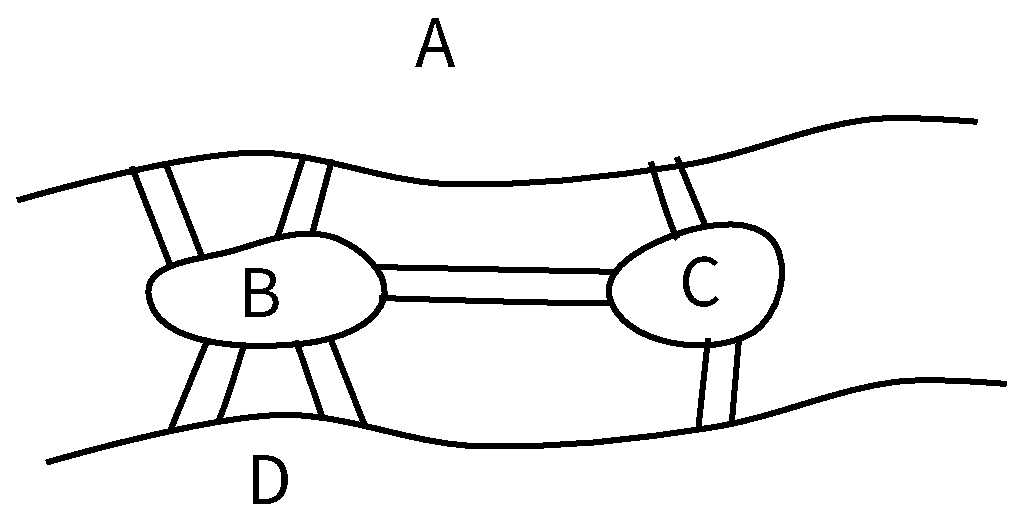
\includegraphics[width=5cm,height=4cm]{konigsberg} 

  \begin{Def}
    包含图的所有顶点和所有边的闭迹称为欧拉闭迹。存在一条欧拉闭迹的图称为欧拉图。
  \end{Def}
  \begin{Thm}
    图G为欧拉图当且仅当$G$为连通的且每个顶点的度为偶数。
  \end{Thm}
  \begin{proof}[证明]
      首先,假设图$G$为欧拉图,往证$G$为连通的且每个顶点的度为偶数。

  由图$G$为欧拉图知$G$中有一条包含所有边和所有顶点的闭迹$T:v_0,x_1,v_1,\ldots,
  x_n,v_n$,其中$v_n=v_0$。显
  然$G$是连通的。顶点$v_0$在$T$中的第一次出现与一条边相关联,最后一次出现与一
  条边相关联,其余的每次出现均与两条边相关联,因此其度为偶数。除$v_0$之外的其他
  顶点在$T$中的每次出现均与两条边相关联,因此其度也为偶数。

  其次,假设$G$为连通的且每个顶点的度为偶数,往证$G$为欧拉图。

  设$v_0,x_1,v_1,\ldots, x_n,v_n$为图$G$的一条最长的迹,记为$Z$,则$Z$为闭迹。否
  则,$v_n \neq v_0$,$v_n$在迹$Z$中的最后一次出现与一条边相关联,其他的每次出现
  均与两条边相关联,由$v_n$的度为偶数知,$v_n$在$G$中还有一条与之关联的边没有在
  $Z$中出现,记为$x_{n+1}=v_nv_{n+1}$。则$v_0,x_1,v_1,\ldots,
  x_n,v_n,x_{n+1},v_{n+1}$构成了图$G$的一条更长的迹,这与$v_0,x_1,v_1,\ldots,
  x_n,v_n$为图$G$的一条最长的迹矛盾。接下来证明$Z$包含了图$G$的所有的边。若不然,
  则图$G$中有一条边$x$不在$Z$中出现,并且$x$有一个端点在$Z$中出现。在图$G$中去掉
  $Z$中的所有边,得到图$G'$。取图$G'$中一条包含$x$的最长的迹$Z'$,由图$G'$中所有
  顶点的度均为偶数易知$Z'$为闭迹(与前面证明$Z$为闭迹的过程相类似)。于是$Z$和
  $Z'$可以联结成一条更长的迹,这与$v_0,x_1,v_1,\ldots, x_n,v_n$为图$G$的一条最长
  的迹矛盾。
  \end{proof}

   \begin{Def}
    包含图的所有顶点和边的迹称为欧拉迹。一条欧拉迹如果不是欧拉闭迹,则称其为欧拉开迹。
  \end{Def}
  \begin{Thm}
    图G有一条欧拉开迹当且仅当$G$为连通的且恰有两个奇度顶点。
  \end{Thm}
  \begin{proof}[证明]
      设图$G$有一条欧拉开迹$Z:v_0,x_1,v_1,\ldots, x_n,v_n$,其中$x_i=v_{i-1}v_i, i =
  1,2,\ldots, n$。显然,图$G$是连通的。顶点$v_0$在$Z$中除了其首次出现与一条边相
  关联外,其余的每次出现均与两
  条边相关联,因此顶点$v_0$的度为奇数;同理,$v_n$的度为奇数。除了$v_0$和$v_n$
  之外其余的每个顶点在$Z$中的每次出现均与两条边相关联,因此其度为偶数。这证明了
  图$G$恰有两个奇度顶点。

  设图$G$是连通的,且恰有两个奇度顶点$u$和$v$。在顶点$u$和$v$之间加一条边,得
  到图$G'$。则图$G'$是连通的且每个顶点的度为偶数,因此有一条欧拉闭迹。在该欧拉闭迹上去掉
  新加的顶点$u$与顶点$v$之间的边,便得到了图$G$的一条欧拉开迹。
  \end{proof}
  \begin{Thm}
    设$G$为连通图,$G$恰有$2n$个奇度顶点,$n \geq 1$,则$G$的全部边可以排成$n$条
    开迹,且不能排成少于$n$条开迹。  \end{Thm}
  \begin{proof}[证明]
      设连通图$G$有$2n$个奇度顶点$u_1,v_1,u_2,v_2,\ldots,u_n,v_n$。在$G$中加
  入$n$条边$u_1v_1$, $u_2v_2$, $\ldots$, $u_nv_n$,得到图$G'$。则$G'$是连通的,
  且每个顶点的度为偶数,因此存在一条欧拉闭迹$Z$。在$Z$中去掉新加入的边$u_1v_1,
  u_2v_2, \ldots, u_nv_n$,则得到图$G$的$n$条开迹。

  假设图$G$的所有边能排成$m$条开迹,$m < n$。则只有这$m$条开迹的端点可能为
  奇度顶点,因此图$G$至多有$2m$个奇度顶点,这与图$G$有$2n$个奇度顶点矛盾。
\end{proof}
   \begin{Def}
    图$G$的一条包含所有顶点的路称为$G$的一条哈密顿路;图$G$的一个包含所有顶点的圈称为$G$的一个哈密顿圈。具有哈密顿圈的图称为哈密顿图。
  \end{Def}  
  \centering
    \begin{tikzpicture}[auto,
    specification/.style ={circle, draw, thick, inner sep = 0pt, minimum size=2mm}]
   \node[specification] (A)  at (18:2.3cm)  {};
   \node[specification] (B)  at (90:2.3cm)  {};
   \node[specification] (C)  at (162:2.3cm)  {};
   \node[specification] (D) at (234:2.3cm)  {};
   \node[specification] (E)  at (306:2.3cm)  {};
   \node[specification] (F)  at (18:1.5cm)  {};
   \node[specification] (G)  at (90:1.5cm)  {};
   \node[specification] (H)  at (162:1.5cm)  {};
   \node[specification] (I) at (234:1.5cm)  {};
   \node[specification] (J)  at (306:1.5cm)  {};
   \node[specification] (K)  at (-18:1.0cm)  {};
   \node[specification] (L)  at (-90:1.0cm)  {};
   \node[specification] (M)  at (-162:1.0cm)  {};
   \node[specification] (N) at (-234:1.0cm)  {};
   \node[specification] (O)  at (-306:1.0cm)  {};
   \node[specification] (P)  at (-18:0.5cm)  {};
   \node[specification] (Q)  at (-90:0.5cm)  {};
   \node[specification] (R)  at (-162:0.5cm)  {};
   \node[specification] (S) at (-234:0.5cm)  {};
   \node[specification] (T)  at (-306:0.5cm)  {};
   
   
   \draw[thick] (A) to  (B);
   \draw[thick] (B) to  (C);
   \draw[thick] (C) to  (D);
   \draw[thick] (D) to  (E);
   \draw[thick] (E) to  (A);
   \draw[thick] (A) to  (F);
   \draw[thick] (B) to  (G);
   \draw[thick] (C) to  (H);
   \draw[thick] (D) to  (I);
   \draw[thick] (E) to  (J);

   \draw[thick] (F) to  (O);
   \draw[thick] (O) to  (G);
   \draw[thick] (G) to  (N);
   \draw[thick] (N) to  (H);
   \draw[thick] (H) to  (M);
   \draw[thick] (M) to  (I);
   \draw[thick] (I) to  (L);
   \draw[thick] (L) to  (J);
   \draw[thick] (J) to  (K);
   \draw[thick] (K) to  (F);

   \draw[thick] (P) to  (K);
   \draw[thick] (Q) to  (L);
   \draw[thick] (R) to  (M);
   \draw[thick] (S) to  (N);
   \draw[thick] (T) to  (O);

   \draw[thick] (P) to  (Q);
   \draw[thick] (Q) to  (R);
   \draw[thick] (R) to  (S);
   \draw[thick] (S) to  (T);
   \draw[thick] (T) to  (P);
 \end{tikzpicture}
 
  \centering
    \begin{tikzpicture}[auto,
    specification/.style ={circle, draw, thick, inner sep = 0pt, minimum size=2mm}]
   \node[specification] (A)  at (30:2.3cm)  {};
   \node[specification] (B)  at (90:2.3cm)  {};
   \node[specification] (C)  at (150:2.3cm)  {};
   \node[specification] (D) at (210:2.3cm)  {};
   \node[specification] (E)  at (270:2.3cm)  {};
   \node[specification] (F)  at (330:2.3cm)  {};
   \node[specification] (G)  at (30:1.5cm)  {};
   \node[specification] (H)  at (90:1.5cm)  {};
   \node[specification] (I) at (150:1.5cm)  {};
   \node[specification] (J)  at (210:1.5cm)  {};
   \node[specification] (K)  at (270:1.5cm)  {};
   \node[specification] (L)  at (330:1.5cm)  {};
   \node[specification] (M)  at (30:0.75cm)  {};
   \node[specification] (N)  at (150:0.75cm)  {};
   \node[specification] (P)  at (270:0.75cm)  {};
   \node[specification] (Q)  at (0,0)  {};
   \draw[thick] (A) to  (B);
   \draw[thick] (B) to  (C);
   \draw[thick] (C) to  (D);
   \draw[thick] (D) to  (E);
   \draw[thick] (E) to  (F);
   \draw[thick] (F) to  (A);
   \draw[thick] (A) to  (G);
   \draw[thick] (B) to  (H);
   \draw[thick] (C) to  (I);
   \draw[thick] (D) to  (J);
   \draw[thick] (E) to  (K);
   \draw[thick] (F) to  (L);
   \draw[thick] (G) to  (H);
   \draw[thick] (H) to  (I);
   \draw[thick] (I) to  (J);
   \draw[thick] (J) to  (K);
   \draw[thick] (K) to  (L);
   \draw[thick] (L) to  (G);
   \draw[thick] (H) to  (M);
   \draw[thick] (M) to  (L);
   \draw[thick] (L) to  (P);
   \draw[thick] (P) to  (J);
   \draw[thick] (J) to  (N);
   \draw[thick] (N) to  (H);
   \draw[thick] (M) to  (Q);
   \draw[thick] (N) to  (Q);
   \draw[thick] (P) to  (Q);
 \end{tikzpicture}

  \begin{Thm}
    设$G=(V,E)$为哈密顿图,则对$V$的每个非空子集$S$,均有
    \[\omega(G-S) \leq |S|\]
    其中$G-S$是从$G$中去掉$S$中那些顶点后所得到的图,$\omega(G-S)$是图$G-S$的支数。
  \end{Thm}
  \centering
    \begin{tikzpicture}[auto,
    specification/.style ={circle, draw, thick, inner sep = 0pt, minimum size=2mm}]
   \node[specification] (A)  at (90:1.6cm)  {};
   \node[specification] (B)  at (210:1.6cm)  {};
   \node[specification] (C)  at (330:1.6cm)  {};
   \node[specification] (D)  at (90:0.8cm)  {};
   \node[specification] (E)  at (210:0.8cm)  {};
   \node[specification] (F)  at (330:0.8cm)  {};
   \node[specification] (G)  at (210:2.4cm)  {};
   \node[specification] (H)  at (330:2.4cm)  {};
   \node[specification] (I)  at (0,0)  {};
   
   
   \draw[thick] (A) to  (B);
   \draw[thick] (B) to  (C);
   \draw[thick] (C) to  (A);
   \draw[thick] (D) to  (E);
   \draw[thick] (E) to  (F);
   \draw[thick] (F) to  (D);
   \draw[thick] (D) to  (G);
   \draw[thick] (D) to  (H);
   \draw[thick] (H) to  (B);
   \draw[thick] (G) to  (C);
   \draw[thick] (A) to  (D);
   \draw[thick] (C) to  (F);
   \draw[thick] (B) to  (E);
   \draw[thick] (I) to  (D);
   \draw[thick] (I) to  (E);
   \draw[thick] (I) to  (F);
   \draw[thick] (G) to  (B);
   \draw[thick] (H) to  (C);
   \draw[thick] (B) to [bend right = 10] (I);
   \draw[thick] (C) to [bend left = 10] (I);
 \end{tikzpicture}
\begin{Thm}
    设$G$为一个有$p$个顶点的图,如果对$G$的每一对不临接的顶点$u$和$v$,均有
    \begin{equation*}
      \deg u + \deg v \geq p - 1,
    \end{equation*}
则$G$为连通的。
\end{Thm}
\begin{proof}[证明]
  用反证法。假设$G$不连通,则$G$至少有两个支。设$G_1=(V_1,E_1)$为其中的一个支,其他各支构成的子图为$G_2=(V_2,E_2)$。取$V_1$中的任意一个顶点$u$和$V_2$中的任意一个顶点$v$,则顶点$u$和顶点$v$不邻接并且
  \[\deg u + \deg v \leq (|V_1| - 1 ) + (|V_2| - 1) = p - 2\]
  矛盾。
\end{proof}
  \begin{Thm}
    设$G$为一个有$p$个顶点的图,如果对$G$的每一对不临接的顶点$u$和$v$,均有
    \begin{equation*}
      \deg u + \deg v \geq p - 1,
    \end{equation*}
则$G$有哈密顿路。
\end{Thm}
\centering
\vspace{0.5cm}
    \begin{tikzpicture}[auto,
    specification/.style ={circle, draw, thick, inner sep = 0pt, minimum size=2mm}]
   \node[specification] (A)  [label=-90:$v_1$] at (0,0)  {};
   \node[specification] (B)  [label=-90:$v_2$] at (0.5,0)  {};
   \node[specification] (C)  at (1,0)  {};
   \node[specification] (D) at (1.5,0)  {};
   \node[specification] (E)  [label=-90:$v_{i_{s-1}}$] at (2,0)  {};
   \node[specification] (F)  [label=-90:$v_{i_s}$]at (2.5,0)  {};
   \node[specification] (G)  at (3,0)  {};
   \node[specification] (H)  at (3.5,0)  {};
   \node[specification] (I) at (4,0)  {};
   \node[specification] (J) [label=-90:$v_{k-1}$] at (4.5,0)  {};
   \node[specification] (K) [label=-90:$v_k$] at (5,0)  {};
   
   
   \draw[thick] (A) to  (B);
   \draw[thick] (B) to  (C);
   \draw[thick] (C) to  (D);
   \draw[thick] (D) to  (E);
   \draw[thick] (E) to  (F);
   \draw[thick] (F) to  (G);
   \draw[thick] (G) to  (H);
   \draw[thick] (H) to  (I);
   \draw[thick] (I) to  (J);
   \draw[thick] (J) to  (K);
%   \draw[thick] (A) to [bend left = 20] (F);
%   \draw[thick] (K) to [bend left = 20] (E);
 \end{tikzpicture}
 \centering
\vspace{0.5cm}
    \begin{tikzpicture}[auto,
    specification/.style ={circle, draw, thick, inner sep = 0pt, minimum size=2mm}]
   \node[specification] (A)  [label=-90:$v_1$] at (0,0)  {};
   \node[specification] (B)  [label=-90:$v_2$] at (0.5,0)  {};
   \node[specification] (C)  at (1,0)  {};
   \node[specification] (D) at (1.5,0)  {};
   \node[specification] (E)  [label=-90:$v_{i_{s-1}}$] at (2,0)  {};
   \node[specification] (F)  [label=-90:$v_{i_s}$]at (2.5,0)  {};
   \node[specification] (G)  at (3,0)  {};
   \node[specification] (H)  at (3.5,0)  {};
   \node[specification] (I) at (4,0)  {};
   \node[specification] (J) [label=-90:$v_{k-1}$] at (4.5,0)  {};
   \node[specification] (K) [label=-90:$v_k$] at (5,0)  {};
   
   
   \draw[thick] (A) to  (B);
   \draw[thick] (B) to  (C);
   \draw[thick] (C) to  (D);
   \draw[thick] (D) to  (E);
   \draw[thick] (E) to  (F);
   \draw[thick] (F) to  (G);
   \draw[thick] (G) to  (H);
   \draw[thick] (H) to  (I);
   \draw[thick] (I) to  (J);
   \draw[thick] (J) to  (K);
   \draw[thick] (A) to [bend left = 20] (F);
   \draw[thick] (K) to [bend left = 20] (E);
 \end{tikzpicture}

 \begin{proof}[证明]\justifying\let\raggedright\justifying
   当$p=1,2,3$时,易验证结论成立。以下证明当$p\geq 4$时结论成立。
    设$G$中的最长路为$v_1v_2\cdots v_k$,只需证明$k = p$。

    用反证法,假设$k < p$,易验证此时$k\geq 3$。以下证明$v_1v_2\cdots v_k$必在同一个圈上。
    % \begin{itemize}
    % \item 如果$v_1$与$v_k$邻接,则$v_1v_2\cdots v_kv_1$构成$G$中的一个圈;
    % \item 如果$v_1$与$v_k$不邻接,由$v_1v_2\cdots v_k$为最长路知$v_1,v_k$只能与$v_2,v_3,\ldots,v_{k-1}$中的顶点邻接。
    % \end{itemize}
由$v_1v_2\cdots v_k$为最长路知$v_1$只能与$v_2,v_3,\ldots,v_{k-1},v_k$中的顶点邻接,$v_k$只能与$v_1,v_2,v_3,\ldots,v_{k-1}$中的顶点邻接。
设$v_{i_1},v_{i_2},\ldots,v_{i_r}$与$v_1$邻接,$2=i_1 < i_2 < \cdots < i_r \leq k$,则$v_k$必与某个$v_{i_s-1}$邻接。
      否则,$v_k$至多与最长路上其余的顶点邻接,所以
      \[\deg v_1 + \deg v_k \leq r + ((k-1) - r) = k - 1 < p - 1\]
      矛盾。于是,$v_1v_2\cdots v_{i_{s-1}}v_kv_{k-1}\cdots v_{i_s}v_1$为$G$中的一个圈。

          由于$G$为连通的,$k < p$,所以$G$必有某个顶点$v$,$v$不在$C$上,但
    与$C$上某个顶点$v_i$邻接。于是得到$G$的一条更长的路,这就出现了矛盾。
\end{proof}
  \begin{Thm}
    设$G$为有$p(p \geq 3)$个顶点的图。如果对$G$的任一对不邻接的顶点$u$和$v$,均有
    \begin{equation*}
      \deg u + \deg v \geq p,
    \end{equation*}
则$G$为一个哈密顿图。
\end{Thm}
\centering
\vspace{0.5cm}
    \begin{tikzpicture}[auto,
    specification/.style ={circle, draw, thick, inner sep = 0pt, minimum size=2mm}]
   \node[specification] (A)  [label=-90:$v_1$] at (0,0)  {};
   \node[specification] (B)  [label=-90:$v_2$] at (0.5,0)  {};
   \node[specification] (C)  at (1,0)  {};
   \node[specification] (D) at (1.5,0)  {};
   \node[specification] (E)  [label=-90:$v_{i_{s-1}}$] at (2,0)  {};
   \node[specification] (F)  [label=-90:$v_{i_s}$]at (2.5,0)  {};
   \node[specification] (G)  at (3,0)  {};
   \node[specification] (H)  at (3.5,0)  {};
   \node[specification] (I) at (4,0)  {};
   \node[specification] (J) [label=-90:$v_{p-1}$] at (4.5,0)  {};
   \node[specification] (K) [label=-90:$v_p$] at (5,0)  {};
   
   
   \draw[thick] (A) to  (B);
   \draw[thick] (B) to  (C);
   \draw[thick] (C) to  (D);
   \draw[thick] (D) to  (E);
   \draw[thick] (E) to  (F);
   \draw[thick] (F) to  (G);
   \draw[thick] (G) to  (H);
   \draw[thick] (H) to  (I);
   \draw[thick] (I) to  (J);
   \draw[thick] (J) to  (K);
%   \draw[thick] (A) to [bend left = 20] (F);
%   \draw[thick] (K) to [bend left = 20] (E);
 \end{tikzpicture}
 \centering
\vspace{0.5cm}
    \begin{tikzpicture}[auto,
    specification/.style ={circle, draw, thick, inner sep = 0pt, minimum size=2mm}]
   \node[specification] (A)  [label=-90:$v_1$] at (0,0)  {};
   \node[specification] (B)  [label=-90:$v_2$] at (0.5,0)  {};
   \node[specification] (C)  at (1,0)  {};
   \node[specification] (D) at (1.5,0)  {};
   \node[specification] (E)  [label=-90:$v_{i_{s-1}}$] at (2,0)  {};
   \node[specification] (F)  [label=-90:$v_{i_s}$]at (2.5,0)  {};
   \node[specification] (G)  at (3,0)  {};
   \node[specification] (H)  at (3.5,0)  {};
   \node[specification] (I) at (4,0)  {};
   \node[specification] (J) [label=-90:$v_{p-1}$] at (4.5,0)  {};
   \node[specification] (K) [label=-90:$v_p$] at (5,0)  {};
   
   
   \draw[thick] (A) to  (B);
   \draw[thick] (B) to  (C);
   \draw[thick] (C) to  (D);
   \draw[thick] (D) to  (E);
   \draw[thick] (E) to  (F);
   \draw[thick] (F) to  (G);
   \draw[thick] (G) to  (H);
   \draw[thick] (H) to  (I);
   \draw[thick] (I) to  (J);
   \draw[thick] (J) to  (K);
   \draw[thick] (A) to [bend left = 20] (F);
   \draw[thick] (K) to [bend left = 20] (E);
 \end{tikzpicture}

     \begin{proof}[证明]
    由定理6.12知,$G$有哈密顿路,记为$v_1v_2\cdots v_p$。

    以下证明$v_1v_2\cdots v_p$必在同一个圈上,从而$G$中有哈密顿圈。

       设$v_{i_1},v_{i_2},\ldots,v_{i_r}$与$v_1$邻接,$2=i_1 < i_2 < \cdots < i_r \leq p$,则$v_p$必与某个$v_{i_s-1}$邻接。
      否则,$v_p$至多与最长路上其余的顶点邻接,所以
      \[\deg v_1 + \deg v_p \leq r + ((p-1) - r) = p - 1\]
      与已知条件矛盾。于是,$v_1v_2\cdots v_{i_{s-1}}v_pv_{p-1}\cdots v_{i_s}v_1$为$G$中的一个圈。
\end{proof}

\begin{Def}
  设$G=(V,E)$为一个图,$V=\{v_1,v_2,\ldots,v_p\}$。$p\times p$矩阵$A=(a_{ij})$称为$G$的邻接矩阵,其中
  \[a_{ij}=\begin{cases}
      1, \text{如果}\{v_i,v_j\}\in E\\
      0, \text{如果}\{v_i,v_j\}\notin E\\
    \end{cases}
  \]
\end{Def}
  \begin{Thm}
    设$G=(V,E)$为一个(p,q)图,$p\times p$矩阵$A$为$G$的邻接矩阵,则$G$中$v_i$与
    $v_j$间长为$l$的通道的条数等于$A^l$的第$i$行第$j$列元素的值。
  \end{Thm}
  \begin{proof}[证明]
      用数学归纳法证明,施归纳于$l$。

  当$l=1$时,结论显然成立。

  假设当$l=k$时结论成立,往证当$l=k+1$时结论也成立。由矩阵乘法的计算规则知:
  \[(A^{k+1})_{ij} = (A^{k}A)_{ij} = \sum_{h=1}^p(A^k)_{ih}A_{hj}\]

  由归纳假设,$(A^k)_{ih}$为从顶点$v_i$到顶点$v_h$长度为$k$的通道的条数。

  由从顶点$v_i$到顶点$v_j$长度为$k+1$的通道的条数为从顶点$v_i$到顶点$v_j$长度为
  $k+1$且倒数第二个顶点依次为$v_1$,$v_2$,$\ldots$,$v_p$的通道的条数之和
  知$(A^{k+1})_{ij}$为从顶点$v_i$到顶点$v_j$长度为$k+1$的通道的条数。
\end{proof}

    \begin{Exercise}
    设$G$是一个$(p,q)$图,证明:
    若$q \geq p + 4$,则$G$中有两个边不重的圈。
  \end{Exercise}
  \begin{Exercise}
    画出具有$4$个顶点的所有无向图(同构的只算一个)。
  \end{Exercise}
    \begin{Exercise}
    在一个有$n$个人的宴会上,每个人至少有$m$个朋友($2 \leq m \leq n$)。试证:
    有不少于$m+1$个人,使得它们按某种方法坐在一张圆桌旁,每人的左右均是他的朋友。
  \end{Exercise}
  \begin{Exercise}
    设$G$是图。证明:若$\delta (G) \geq 2$,则$G$包含长至少为$\delta (G) + 1$的
    圈。
  \end{Exercise}
  \begin{Exercise}
      若$G$是一个$(p,q)$图,$q > \frac{1}{2}(p-1)(p-2)$,试证$G$为连通图。  
    \end{Exercise}
    \begin{Exercise}
      菱形12面体的表面上有无哈密顿圈?
      
  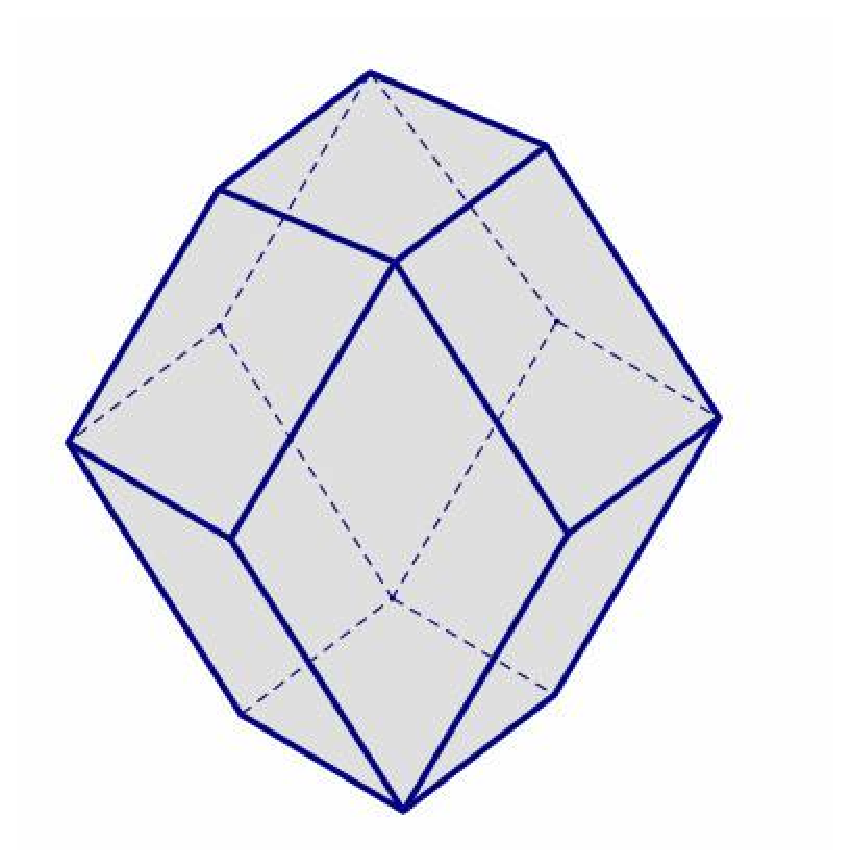
\includegraphics[width=5cm,height=4cm]{timg}  
\end{Exercise}

\setcounter{Exercise}{0}
    \begin{Exercise}
    设$G$是一个$(p,q)$图,证明:
    若$q \geq p + 4$,则$G$中有两个边不重的圈。
  \end{Exercise}

  \begin{proof}[证明]
    当$q > p + 4$时,可以在$G$中任意去掉一些边,使得剩余的边数恰好比顶点数多4。如果此时
    得到的新图中有两个边不重的圈,则原来的图$G$中也一定有两个边不重的圈。因此,
    以下只需证当$q=p+4$时,图$G$中有两个边不重的圈。

    用数学归纳法证明,施归纳于顶点数$p$。

    (1)当$p \leq 4$时,图$G$最多有$p(p-1)/2$条边,易验证此时$q = p + 4$不可能成
    立。当$p = 5$时,$q = 9$。设此时图
    $G$的顶点集为$\{v_1,v_2,v_3,v_4,v_5\}$,除了$v_1$和$v_5$之间没有边关联之外,其余的任意两
    个顶点之间均有边关联,则此时$v_1v_2v_3v_1$和$v_3v_4v_5v_3$就是图$G$中两个边不重的
    圈。

       (2)假设当$p = k$时结论成立,往证当$p = k+1$时结论也成立。设图$G$有$k+1$个顶点。
    分以下四种情况进行验证:

    
    (i)当$\delta(G)=0$时,去掉图$G$中任意一个度为0的顶点和任意一条边,得到的图
    $G'$中有$p'$个顶点,$q'$条边,则$q'=p'+4$。由归纳假设,图$G'$中有两个边不重的圈,它们也是图
    $G$中两个边不重的圈。

    (ii)当$\delta(G)=1$时,去掉图$G$中任意一个度为1的顶点及其与之关联的边,得到
    的图$G'$中有$p'$个顶点,$q'$条边,则$q' = p' + 4$。由归纳假设,图$G'$中有两
    个边不重的圈,它们也是图$G$中两个边不重的圈。

     (iii)当$\delta(G)=2$时,设$u$为图$G$中度为2的顶点,与之邻接的两个顶点为$v$和$w$。分两种情况讨论。在第一种情况下,$v$和$w$之间没有边关联,去掉顶点$u$及其与之关联的两条边$uv$和$uw$,添加一条边$vw$,得到的图$G'$中有$p'$个顶点,$q'$条边,则$q'=p'+4$。由归纳假设,图$G'$中有两个边不重的圈。如果新添加的边$vw$不在这两个圈上,则这两个圈就是图$G$中两个边不重的圈;如果新添加的边$vw$在其中的一个圈上,将其替换为图$G$中的两条边$vu$和$uw$,则所得到的圈与另一个圈一起构成图$G$中两个边不重的圈。在第二种情况下,$v$和$w$之间有边关联,此时$uvwu$构成图$G$中的一个圈,去掉该圈上的三条边,得到的图$G'$中有$p'$个顶点,$q'$条边。此时$q'=p'+1$,因此图$G'$中必定有一个圈,与原来图$G$中的圈$uvwu$构成图$G$中两个边不重的圈。

         (iv)当$\delta(G)\geq 3$时,$2q\geq 3p$,即$2(p+4) \geq 3p$, 可以得到$p \leq
    8$。此时若图$G$中有长度小于等于$4$的圈,将其上的4条边去掉,得到的图$G'$中有
    $p'$个顶点,$q'$条边,则$q'\geq p'$,图$G'$中必定有一个圈,与原来图$G$中去掉的边
    所构成的圈一起构成图$G$中两个边不重的圈。若图$G$中所有圈的长度至少为$5$,设
    $C$为其中长度最短的一个圈。由$\delta(G)\geq 3$知圈$C$上的每
    个顶点至少与圈外的一个顶点相邻接,而其中任意两个不同的顶点不能同时与圈外同一
    个顶点相邻接,否则将产生一个长度更小的圈。由圈$C$上至少有5个顶点知图$G$中至
    少有$10$个顶点,与$p \leq 8$矛盾。这说明图$G$中所有圈的长度至少为$5$的情况不
    可能出现。


  \end{proof}
  

  \cite{Dijkstra} \cite{Shapley} \cite{Kruskal} \cite{Prim} 
  \bibliographystyle{plain}
  \bibliography{ref}

      \chapter{}

\end{CJK*}
\end{document}





%%% Local Variables:
%%% mode: latex
%%% TeX-master: t
%%% End:



